% Bachelor's thesis, UniME L-31 Computer Science, curriculum Data Analysis.
% Build: latexmk -pdf main.tex   (or Overleaf: upload this folder + reports/figures/)
\documentclass[12pt,a4paper,oneside]{report}

\usepackage[T1]{fontenc}
\usepackage[utf8]{inputenc}
\usepackage[english]{babel}
\usepackage[margin=2.5cm]{geometry}
\usepackage{graphicx}
\usepackage{booktabs}
\usepackage{amsmath,amssymb}
\usepackage{siunitx}
\usepackage{caption}
\usepackage[numbers,sort&compress]{natbib}
\usepackage[hidelinks]{hyperref}

% Figures come straight from the analysis outputs; new drawings go in figures/.
\graphicspath{{../reports/figures/}{figures/}}

\usepackage{xcolor}
\newcommand{\todo}[1]{\textcolor{red}{[TODO: #1]}}

\begin{document}

\pagenumbering{roman}
\begin{titlepage}
\centering
{\Large Università degli Studi di Messina\par}
\vspace{1cm}
{\large DIPARTIMENTO DI SCIENZE MATEMATICHE E INFORMATICHE,\\
SCIENZE FISICHE E SCIENZE DELLA TERRA\par}
\vspace{0.5cm}
{\large Bachelor's Degree in Computer Science L31\\
Curriculum: Data Analysis\par}
\vspace{3cm}
{\huge\bfseries Death before Age One among U.S. Live Births:\\[0.3em]
Prediction and Maternal Risk Factors\\[0.3em]
in Linked Birth--Infant Death Cohorts, 2016--2023\par}
\vfill
\begin{minipage}[t]{0.45\textwidth}
\raggedright Supervisor:\\ Prof. Daniele Rav\`{\i}
\end{minipage}\hfill
\begin{minipage}[t]{0.45\textwidth}
\raggedleft Candidate:\\ Elzar Shakulov
\end{minipage}
\vspace{2cm}

Academic Year \todo{confirm with the course office: 2025/2026 or 2026/2027}
\end{titlepage}

\tableofcontents
\listoffigures
\listoftables
\chapter*{Abstract}
\addcontentsline{toc}{chapter}{Abstract}
% One page. Write last. Data, two questions, main numbers, one-line conclusion.
\todo{Data: CDC/NVSS linked birth--infant death cohorts 2016--2023, 29.9 million births, 166,367 deaths.}
\todo{RQ1: best model PR-AUC 0.038 (strict 0.030), ROC-AUC 0.74, test years 2022--2023.}
\todo{RQ2: adjusted RRs: diabetes 1.84, smoking 1.68, BMI $\geq$40 1.53, hypertension 1.50, interval $<$6 months 1.22.}
\todo{Robustness: pre-registered checks, negative control, multiple imputation.}

\chapter*{Acknowledgement}
\addcontentsline{toc}{chapter}{Acknowledgement}
\todo{Write.}


\cleardoublepage
\pagenumbering{arabic}
\chapter{Introduction}
\label{ch:intro}

\section{Background and Motivation}
% U.S. infant mortality 5.35--5.80 per 1,000 (2016--2023); pre-pregnancy hypertension
% 1.7% -> 3.2% (2016 -> 2023), obesity rising (notebooks/02_table1).
\todo{Write.}

\section{Problem Statement}
\todo{Write.}

\section{Research Questions and Objectives}
% RQ1 (prediction): how well can information known before delivery predict death before age one in later cohorts?
% RQ2 (association): after adjustment for confounders, how much do pre-pregnancy hypertension, diabetes,
% BMI class, smoking before pregnancy and the interval since the last pregnancy change the risk?
\todo{Write.}

\section{Thesis Structure}
\todo{One paragraph per chapter.}

\chapter{State of the Art}
\label{ch:sota}

\section{Measuring Infant Mortality}
% NVSS linked birth--infant death files; birth-cohort vs period files; no geography since 2005.
\todo{Write.}

\section{Maternal Risk Factors for Infant Death}
% Hypertension, diabetes, BMI, smoking before pregnancy, interpregnancy interval.
\todo{Write.}

\section{Prediction of Rare Outcomes}
% PR-AUC vs ROC-AUC under a 0.55% base rate \citep{saito2015}; calibration; time shift; decision curves \citep{vickers2006}.
\todo{Write.}

\section{Causal Inference from Observational Data}
% DAGs and the back-door criterion \citep{pearl2009}; collider bias and the birth-weight paradox \citep{hernandezdiaz2006};
% negative controls \citep{lipsitch2010}.
\todo{Write.}

\section{Statistical Tools}
% Modified Poisson \citep{zou2004}; random-effects pooling \citep{dersimonian1986}; E-value \citep{vanderweele2017};
% multiple imputation \citep{rubin1987}.
\todo{Write.}

\chapter{Material and Methods}
\label{ch:methods}

\section{Data Source and Study Population}
% 8 birth cohorts 2016--2023; join on CO_SEQNUM + CO_YOD; RESTATUS < 4; 29,882,341 births, 166,367 deaths.
% Source: AGENTS.md, notebooks/00_data_build.
\todo{Write.}

\section{Data Build and Validation}
% Layouts parsed from the CDC user guides; Parquet build; benchmark vs guide counts and Documentation Table 2.
% Source: notebooks/00_data_build, 01_benchmark; reference/benchmark_*.csv.
\todo{Write.}

\section{Descriptive Analysis and Missing Data}
% Source: notebooks/02_table1; reports/table1_*.csv.
\todo{Write.}

\section{Pre-Registered Analysis Plan}
% plan/analysis_plan.md v1.0 (23 Nov 2026), pass/fail rules fixed before results, dated change log.
\todo{Write.}

\section{Part 1: Prediction}
\subsection{Input Sets}
% Set A (early pregnancy), Set B (before delivery); excluded items and why.
\subsection{Validation Protocol}
% Train 2016--2020 (all deaths + 1 in 10 survivors, weight 10), tune 2021, test 2022--2023 once.
\subsection{Models}
% (a) base rate, (b) age + race logistic, (c) penalized logistic, (d) histogram gradient boosting.
% Limitation: 3-setting grid, best at the edge (GitHub issue #5).
\subsection{Metrics and Uncertainty}
% PR-AUC (main), ROC-AUC, Brier, calibration; 1,000 Poisson bootstrap resamples.
\subsection{Importance and Timing Leakage}
% Grouped permutation importance; strict model without precare, illb, ilp (issue #4: more timing items remain).
\subsection{Neonatal and Postneonatal Models}
\todo{Write all subsections. Source: notebooks/03_prediction, notes/03_prediction_explained.md.}

\section{Part 2: Association}
\subsection{Exposures and Outcomes}
% Gestational age from COMBGEST: justify or add OEGest_Comb sensitivity (issue #3).
\subsection{Confounder Selection with DAGs}
\subsection{Modified Poisson Regression on Pattern Counts}
\subsection{Pooling over Cohorts and Absolute Effects}
\subsection{Pre-Set Checks}
% Direction, heterogeneity, negative control, collider demonstration, missing data.
\subsection{Multiple Imputation and Sensitivity Analyses}
\todo{Write all subsections. Source: notebooks/04_association.}

\section{Extra Analyses (Post-Hoc)}
% E1 cause of death, E2 recording bias, E3 stillbirths, E4 mediation, E5 decision curves, E6 external BMI check.
% Source: notebooks/06_extra_research; plan change log 25 Nov 2026.
\todo{Write.}

\section{Software and Reproducibility}
% Python 3.12, DuckDB, Polars, scikit-learn, statsmodels; requirements.lock; seed 20261123; notebooks 00--06.
\todo{Write.}

\chapter{Results and Discussion}
\label{ch:results}

\section{Data Validation against CDC}
% Counts: deaths 8/8, births 7/8 (2020 guide typo) -> FAIL by rule; Table 2 exact 2018--2023.
\todo{Write. Table: reference/benchmark_counts.csv.}

\section{Who Dies before Age One}
\begin{figure}[htbp]
  \centering
  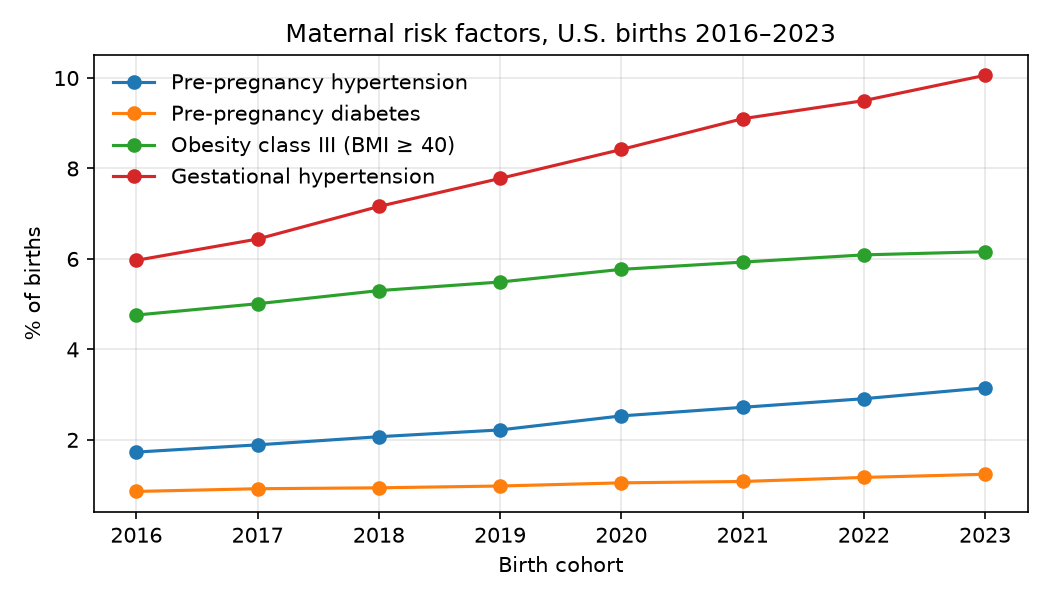
\includegraphics[width=0.85\textwidth]{risk_factor_trends.png}
  \caption{\todo{Caption that states the result.}}
  \label{fig:trends}
\end{figure}
\todo{Write. Table: reports/table1_by_outcome.csv.}

\section{Model Comparison and Calibration}
% Lead with the strict results (0.030; strict-2 0.0275) next to the pre-registered 0.038.
\begin{figure}[htbp]
  \centering
  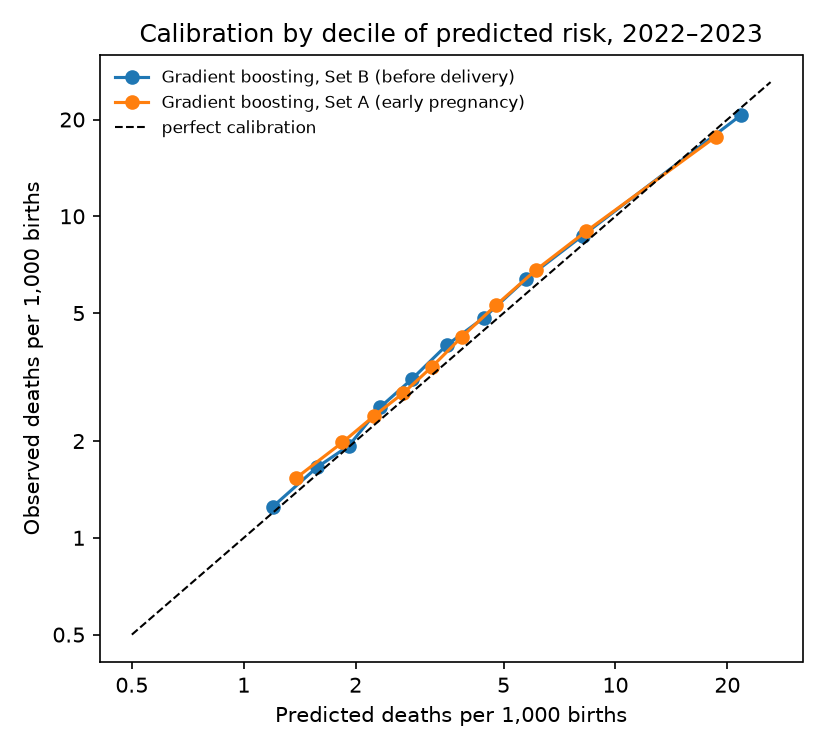
\includegraphics[width=0.75\textwidth]{part1_calibration.png}
  \caption{\todo{Caption.}}
  \label{fig:calibration}
\end{figure}
\todo{Write. Tables: reports/part1_model_comparison.csv, part1_strict.csv, part1_test_years.csv.}

\section{What Drives the Prediction}
\begin{figure}[htbp]
  \centering
  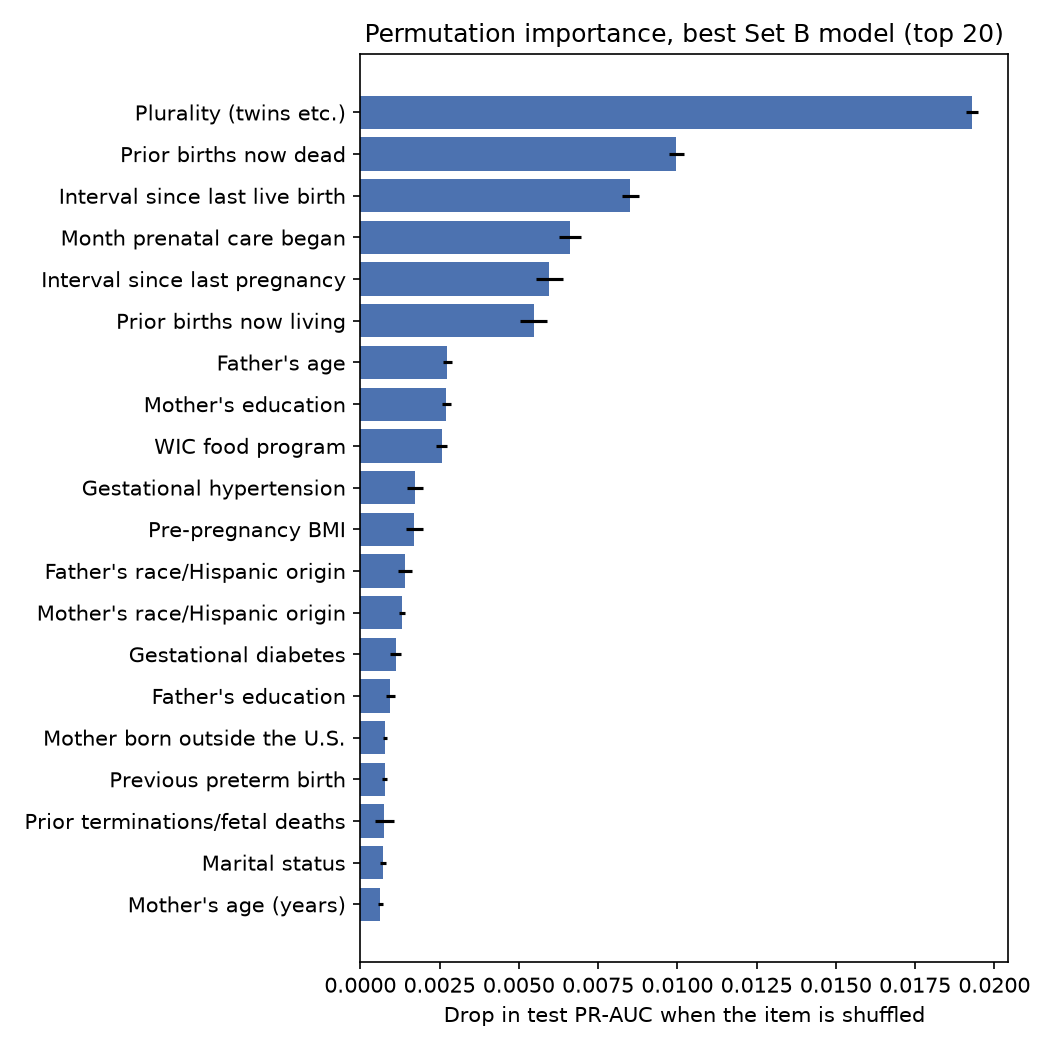
\includegraphics[width=0.85\textwidth]{part1_importance.png}
  \caption{\todo{Caption.}}
  \label{fig:importance}
\end{figure}
\todo{Write. Tables: reports/part1_importance.csv, part1_dropgroup.csv, part1_leakage.csv.}

\section{Early versus Late Deaths, Subgroups and Fairness}
\todo{Write. Tables: reports/part1_agesplit_*.csv, part1_subgroups.csv.}

\section{Decision Curves}
\begin{figure}[htbp]
  \centering
  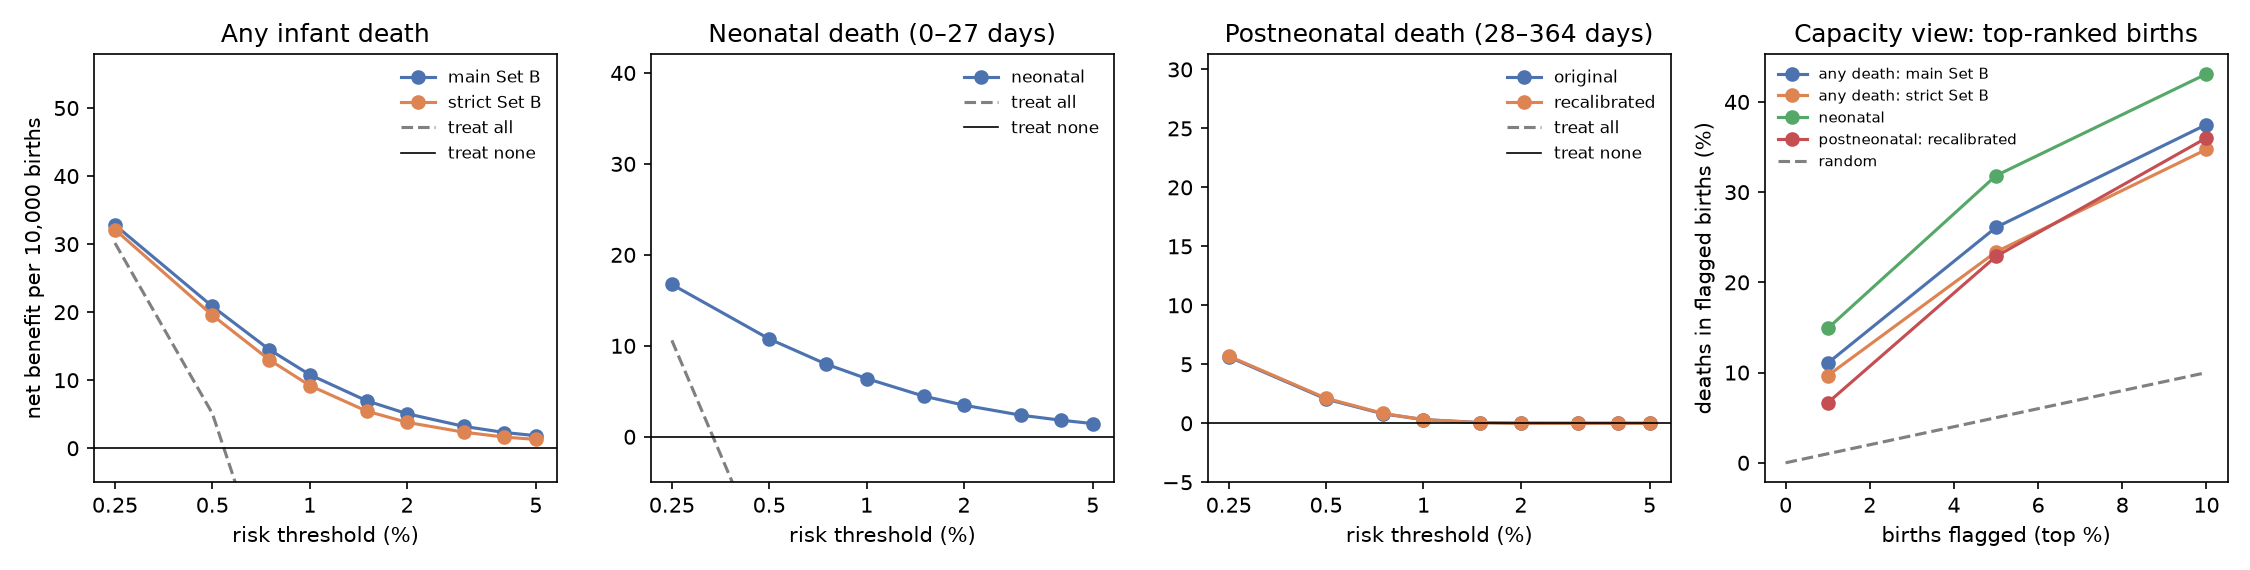
\includegraphics[width=0.85\textwidth]{extra_decision_curves.png}
  \caption{\todo{Caption.}}
  \label{fig:dca}
\end{figure}
\todo{Write. Table: reports/extra_decision_curves.csv.}

\section{Adjusted Risk Ratios for the Five Maternal Factors}
\begin{figure}[htbp]
  \centering
  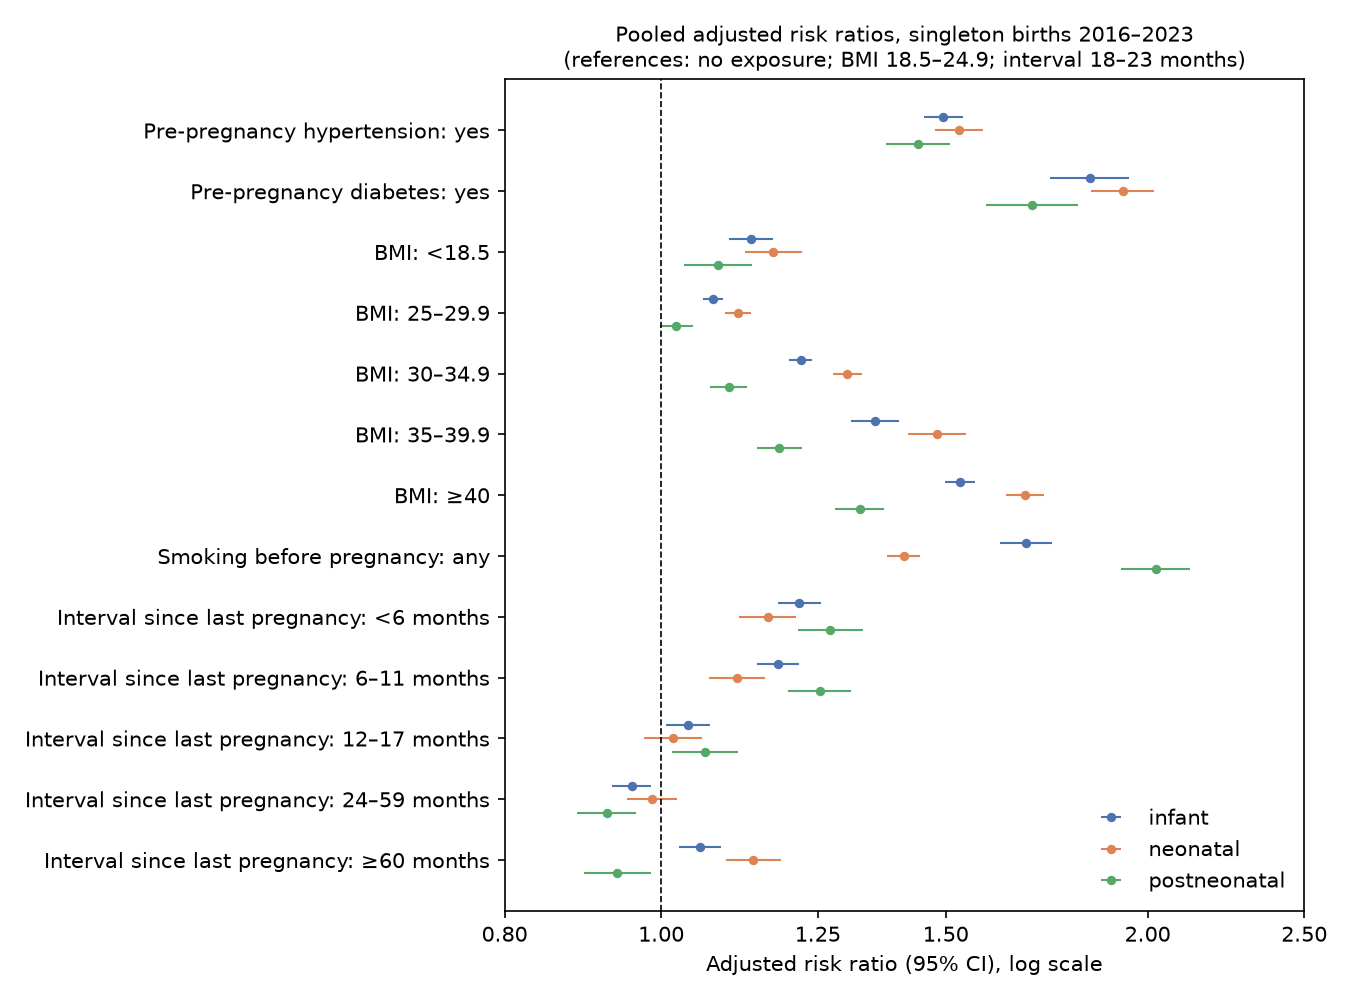
\includegraphics[width=0.85\textwidth]{part2_forest_pooled.png}
  \caption{\todo{Caption.}}
  \label{fig:forest}
\end{figure}
\todo{Write. Tables: reports/part2_results.csv, part2_exposure_counts.csv.}

\section{Robustness: Direction, Heterogeneity, Imputation and Sensitivity}
\todo{Write. Tables: reports/part2_mi_results.csv, part2_sensitivity.csv, part2_social_sensitivity.csv; figure part2_forest_by_cohort.png.}

\section{Negative Control and Collider Demonstration}
% Audit #2 (04 section 19): without codes 148--150 the smoking accident RR is still 1.59 (1.33--1.89).
\todo{Write. Tables: reports/part2_negative_control.csv, part2_collider.csv.}

\section{Cause of Death, Recording Bias and Stillbirths}
\begin{figure}[htbp]
  \centering
  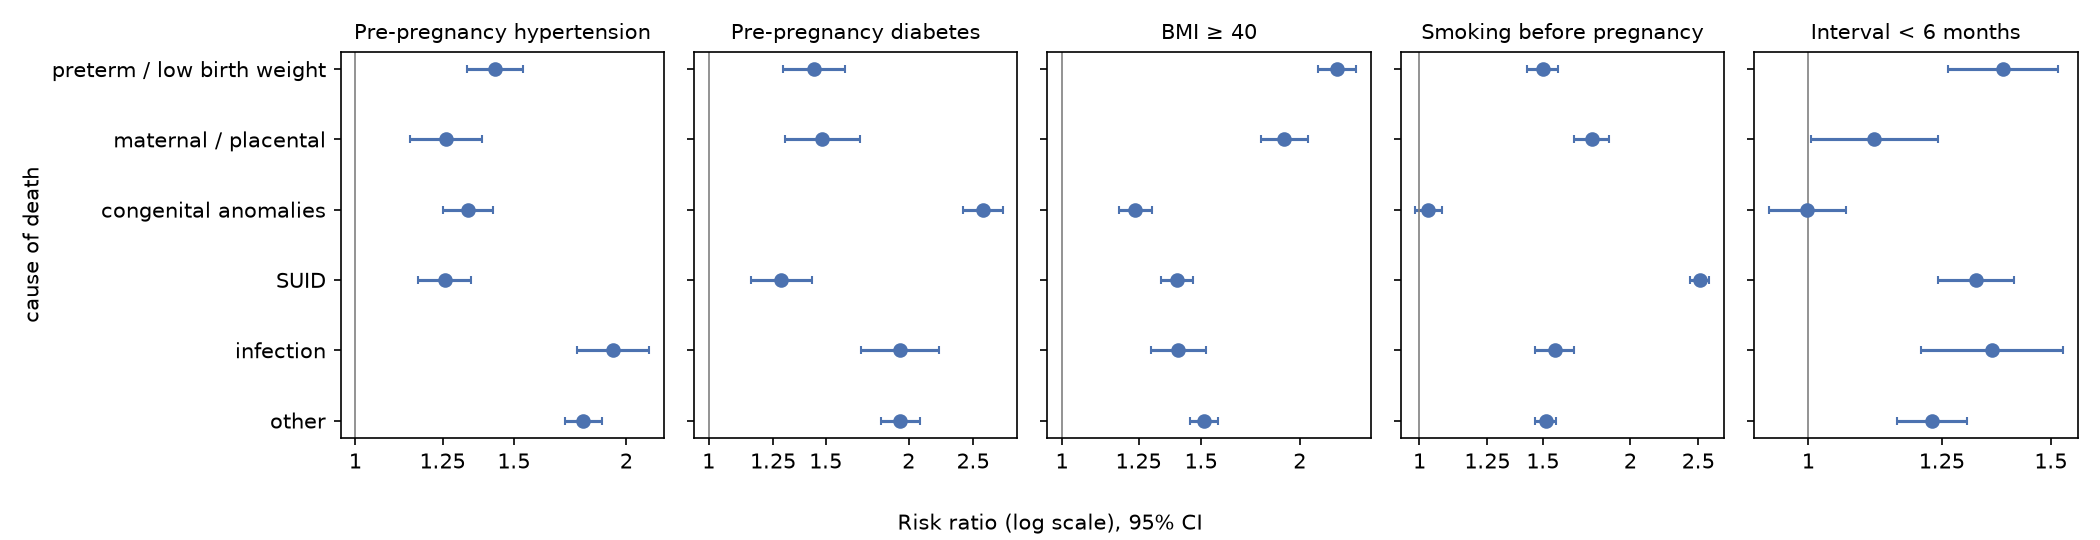
\includegraphics[width=0.85\textwidth]{extra_cause_specific.png}
  \caption{\todo{Caption.}}
  \label{fig:cause}
\end{figure}
\todo{Write. Tables: reports/extra_cause_*.csv, extra_bias_analysis.csv, extra_stillbirth.csv.}

\section{Mediation through Gestational Age}
% Audit #1 (06 section 9): report proportions mediated as upper bounds; OE hypertension direct RR 0.92 < 1.
\todo{Write. Table: reports/extra_mediation.csv.}

\section{Comparison with Published Studies}
\todo{Write.}

\chapter{Conclusion and Future Works}
\label{ch:conclusion}

\section{Summary of Contributions}
\todo{Write.}

\section{Key Findings}
\todo{Write.}

\section{Limitations}
% notes/results_overview.md Part III B and E (audit #1-#5): mediation shares are upper bounds; COMBGEST vs OE.
\todo{Write.}

\section{Future Works}
% County analysis with CDC WONDER + AHRF/ACS; DHS/MICS comparison; obstetric gestational-age estimate.
\todo{Write.}


\bibliographystyle{unsrtnat}
\bibliography{references}

\appendix
\chapter{Pre-Set Checks}
\label{app:a_checks}
% Source: reports/checks.csv
\todo{Fill.}

\chapter{Variables and Codes}
\label{app:b_variables}
% Source: reference/columns.csv
\todo{Fill.}

\chapter{Causal Diagrams}
\label{app:c_dags}
% Source: plan/dags/*.dagitty
\todo{Fill.}

\chapter{Analysis Plan Change Log}
\label{app:d_change_log}
% Source: plan/analysis_plan.md, change log
\todo{Fill.}


\end{document}
